\documentclass[tikz]{standalone}

\usepackage{bm}

\usepackage{tikz}

\usetikzlibrary{patterns}
\usetikzlibrary{circuits.ee.IEC}
\usetikzlibrary{angles, quotes}
\usetikzlibrary{decorations.markings}
\tikzset{>=latex}
\tikzset{->-/.style={decoration={
  markings,
  mark=at position .5 with {\arrow{>}}},postaction={decorate}}}
\tikzset{-<-/.style={decoration={
  markings,
  mark=at position .5 with {\arrow{<}}},postaction={decorate}}}
\usetikzlibrary{decorations.pathmorphing}

\newcommand{\abs}[1]{\left| #1 \right|}
\renewcommand*{\i}{\mathrm{i}}
\renewcommand*{\r}{\mathrm{r}}
\renewcommand*{\t}{\mathrm{t}}
\renewcommand*{\d}{\mathrm{d}}

\begin{document}

\label{E of plane}
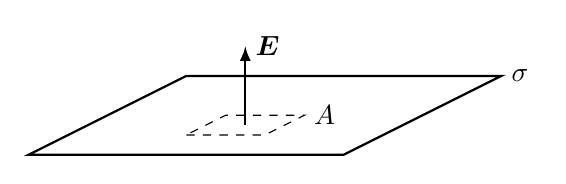
\begin{tikzpicture}
    \draw[thick](0, 0)--(4, 0)--(6, 1)node[right]{$\sigma$}--(2, 1)--cycle;
    \draw[dashed, shift={(2, 0.25)}](0, 0)--(1, 0)--(1.5, .25)node[right]{$A$}--(.5, .25)--cycle;
    % \draw[shift={(2, 0.35)}](0, 0)--(1, 0)--(1.5, .25)--(.5, .25)--cycle;
    % \draw[dashed, shift={(2, 0.15)}](0, 0)--(1, 0)--(1.5, .25)--(.5, .25)--cycle;
    \draw[thick, ->, shift={(2.75, 0.375)}](0, 0)--(0, 1)node[right]{$\bm E$};
\end{tikzpicture}

\label{E of line}
\begin{tikzpicture}
    \draw[thick](-3, 0)--(3, 0)node[right]{$\lambda$};
    \draw[dashed, yshift=.2cm](-.5, 0)--(.5, 0);
    \draw[dashed, yshift=-.2cm](-.5, 0)--(.5, 0);
    \draw[dashed](.5, 0)ellipse(.1 and .2);
    \draw[dashed](-.5, 0)ellipse(.1 and .2);
    \draw[thick, ->, yshift=.2cm](0, 0)--(0, 1)node[right]{$\bm E$};
\end{tikzpicture}

\label{E of half circle}
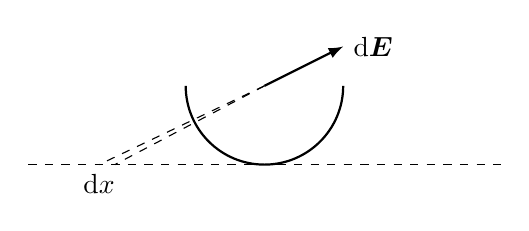
\begin{tikzpicture}
    \draw[thick](-1, 0)arc(-180:0:1);
    \draw[dashed](-3, -1)--(3, -1);
    \draw[dashed](0, 0)--(-2-.1, -1)node[below]{$\d x$};
    \draw[dashed](0, 0)--(-2+.1, -1);
    \draw[thick, ->](0, 0)--(1, .5)node[right]{$\d\bm E$};
\end{tikzpicture}

\label{Phi of sphere conductor}
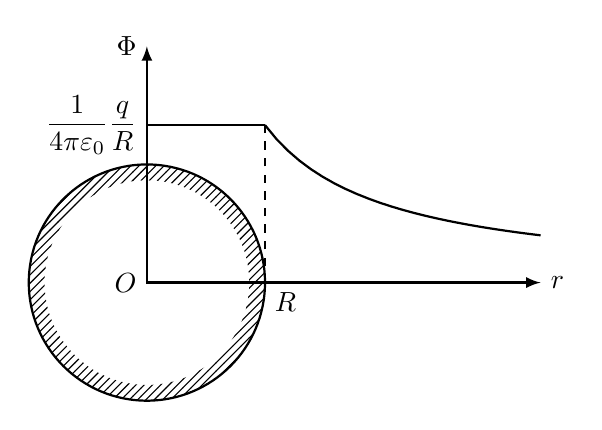
\begin{tikzpicture}[even odd rule]
    \fill[pattern=north east lines](0, 0)circle(1.3)(0, 0)circle(1.5);
    \draw[thick](0, 0)node[left]{$O$}circle(1.5);
    \draw[thick, <->](0, 3)node[left]{$\Phi$}--(0, 0)--(5, 0)node[right]{$r$};
    \draw[dashed](1.5, 0)node[below right]{$R$}--(1.5, 2);
    \draw[thick](0, 2)node[left]{$\displaystyle\frac1{4\pi\varepsilon_0}\frac qR$}--(1.5, 2);
    \draw[thick, domain=1.5:5]plot(\x, {3/\x});
\end{tikzpicture}

\label{E between surfaces}
\begin{tikzpicture}
    \draw[thick](-3, 0)node[below right]{1}node[above right]{2}--(3, 0)node[right]{$\sigma$};
    \draw[thick, ->](0, 0)--(0, 1)node[right]{$\hat{\bm n}$};
    \draw[dashed](0, 2)--(0, -2);
    \draw[thick, ->](-2, -1)node[left]{$\bm E_1$}--(0, 0);
    \draw[thick, ->](0, 0)--(2, 1.5)node[right]{$\bm E_2$};
\end{tikzpicture}

\label{dipole layers}
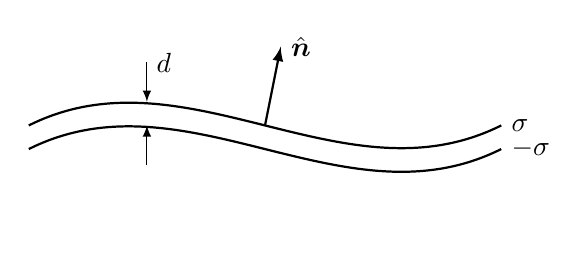
\begin{tikzpicture}[xscale=2]
    \draw[thick](0, 0).. controls (1, 1) and (2, -1) .. (3, 0)node[right]{$\sigma$};
    \draw[thick, yshift=-.3cm](0, 0).. controls (1, 1) and (2, -1) .. (3, 0)node[right]{$-\sigma$};
    \draw[->, shift={(.75, 0)}](0, -.5)--(0, 0);
    \draw[->, shift={(.75, .3)}](0, .5)node[right]{$d$}--(0, 0);
    \draw[thick, ->, xshift=1.5cm](0, 0)--(.1, 1)node[right]{$\hat{\bm n}$};
\end{tikzpicture}

\label{method of images, plane}
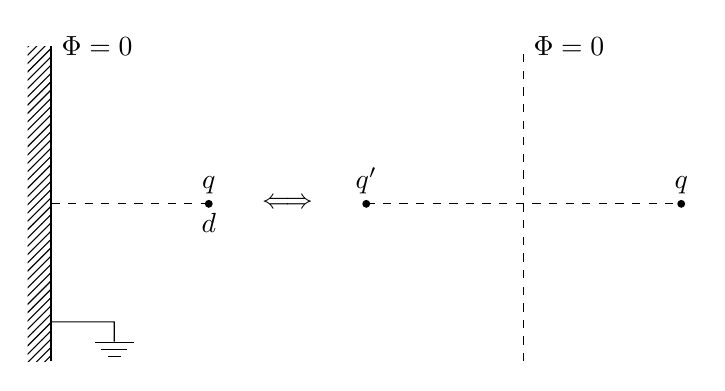
\begin{tikzpicture}[circuit ee IEC]
    \begin{scope}
        \fill[pattern=north east lines](-.3, 0)rectangle(0, 4);
        \draw[thick](0, 0)--(0, 4)node[right]{$\Phi=0$};
        \draw (0, 0.5) to (0.8, 0.5) to [ground={at end}] (0.8, 0.15);
        \draw[dashed](0, 2)--(2, 2)node[below]{$d$};
        \fill[black](2, 2)circle(.05)node[above]{$q$};
    \end{scope}
    \node at (3, 2) {$\iff$};
    \begin{scope}[xshift=6cm]
        \draw[dashed](0, 0)--(0, 4)node[right]{$\Phi=0$};
        \draw[dashed](-2, 2)--(2, 2);
        \fill[black](2, 2)circle(.05)node[above]{$q$};
        \fill[black](-2, 2)circle(.05)node[above]{$q'$};
    \end{scope}
\end{tikzpicture}

\label{method of images, sphere}
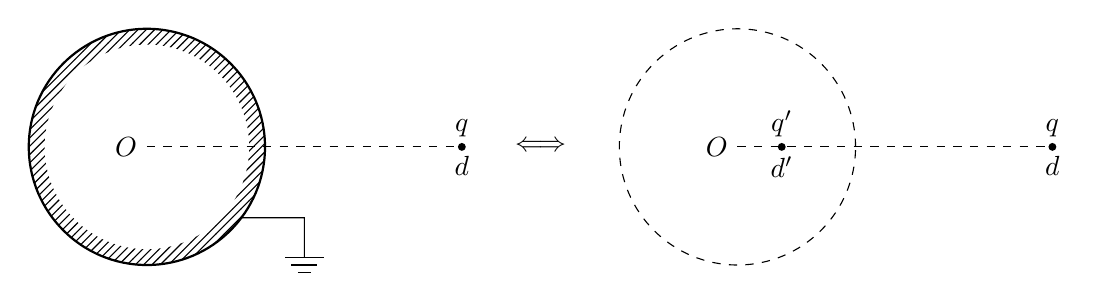
\begin{tikzpicture}[circuit ee IEC]
    \begin{scope}
        \fill[even odd rule, pattern=north east lines](0, 0)circle(1.5)(0, 0)circle(1.3);
        \draw[thick](0, 0)circle(1.5);
        \draw (1.2, -.9) to (2, -.9) to [ground={at end}] (2, -1.5);
        \draw[dashed](0, 0)node[left]{$O$}--(4, 0);
        \fill[black](4, 0)circle(.05)node[below]{$d$}node[above]{$q$};
    \end{scope}
    \node at (5, 0) {$\iff$};
    \begin{scope}[xshift=7.5cm]
        \draw[dashed](0, 0)circle(1.5);
        \draw[dashed](0, 0)node[left]{$O$}--(4, 0);
        \fill[black](4, 0)circle(.05)node[below]{$d$}node[above]{$q$};
        \fill[black](.5625, 0)circle(.05)node[below]{$d'$}node[above]{$q'$};
    \end{scope}
\end{tikzpicture}

\label{uniform E approx pm q}
\begin{tikzpicture}
    \draw[loosely dash dot](-5, 0)--(5, 0);
    \fill[black](4, 0)circle(.05)node[above]{$-Q$}node[below]{$+R$};
    \fill[black](-4, 0)circle(.05)node[above]{$+Q$}node[below]{$-R$};
    \draw[dashed](-4, 0)--(0, .8)--(4, 0);
    %\draw[thick, <->](1, 1)--(0, .8)--(1, .6);
    \draw[thick, ->](0, .8)--(2, .8)node[above]{$\bm E_0$};
\end{tikzpicture}

\label{2 hemisphere}
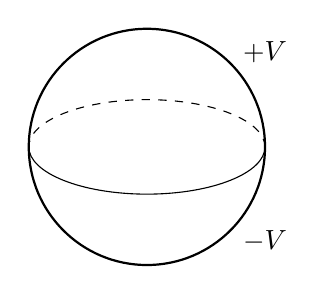
\begin{tikzpicture}[scale=.6]
    \draw[thick](0, 0)circle(2.5);
    \draw[dashed](2.5, 0)arc(0:180:2.5 and 1);
    \draw(-2.5, 0)arc(-180:0:2.5 and 1);
    \node at(2.5, 2){$+V$};
    \node at(2.5, -2){$-V$};
\end{tikzpicture}

\label{3D rectangular box}
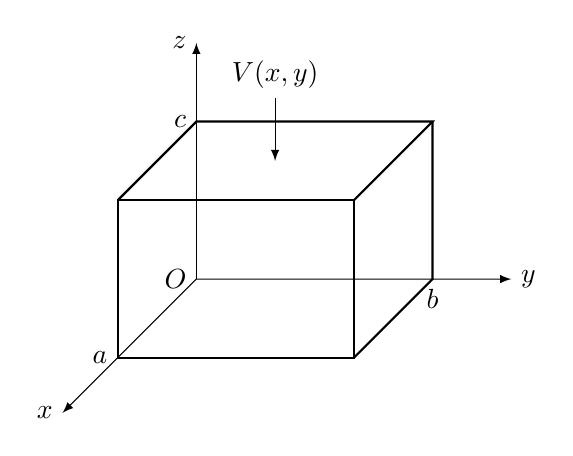
\begin{tikzpicture}
    \draw[thick](0, 0)node[left]{$a$}rectangle(3, 2);
    \draw[thick](0, 2)--(1, 3)node[left]{$c$}--(4, 3)--(3, 2);
    \draw[thick](4, 3)--(4, 1)node[below]{$b$}--(3, 0);
    \draw[<->](5, 1)node[right]{$y$}--(1, 1)node[left]{$O$}--(-.7, -.7)node[left]{$x$};
    \draw[->](1, 1)--(1, 4)node[left]{$z$};
    \draw[->](2, 3.3)node[above]{$V(x,y)$}--(2, 2.5);
\end{tikzpicture}

\label{2D rectangular hole}
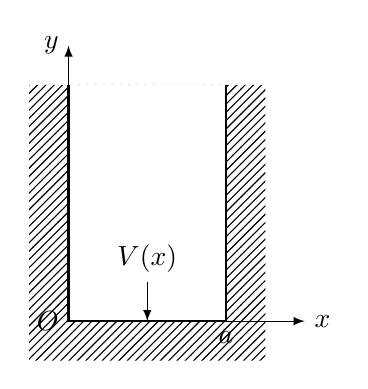
\begin{tikzpicture}[even odd rule]
    \coordinate (O) at (0, 0);
    \fill[pattern=north east lines](-.5, -.5)rectangle(2.5, 3)(O)rectangle(2, 3);
    \draw[<->](3, 0)node[right]{$x$}--(O)node[left]{$O$}--(0, 3.5)node[left]{$y$};
    \draw[thick](0, 3)--(O)--(2, 0)node[below]{$a$}--(2, 3);
    \draw[<-](1, 0)--(1, 0.5)node[above]{$V(x)$};
\end{tikzpicture}

\label{2D angular boundary}
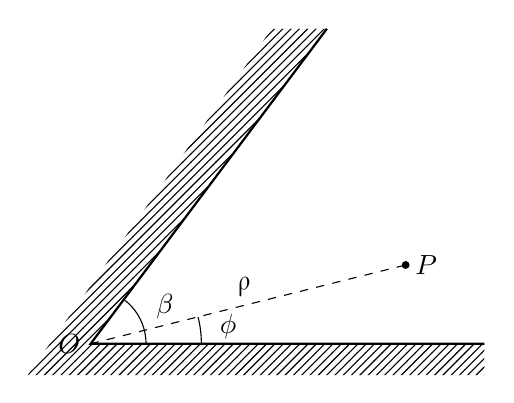
\begin{tikzpicture}
    \coordinate (o) at (0, 0);
    \coordinate (p) at (4, 1);
    \coordinate (a) at (5, 0);
    \coordinate (b) at (3, 4);
    \fill[pattern=north east lines](2.3, 4)--(b)--(o)--(a)--(5, -.4)--(-.8, -.4);
    \draw[thick](b)--(o)node[left]{$O$}--(a);
    \draw[dashed](o)--(p)node[right]{$P$}node[midway, above, sloped]{$\rho$};
    \fill(p)circle(.05);
    \pic[draw, angle radius=20, angle eccentricity=1.5, "$\beta$"]{angle=a--o--b};
    \pic[draw, angle radius=40, angle eccentricity=1.25, "$\phi$"]{angle=a--o--p};
\end{tikzpicture}

\label{2D conical boundary}
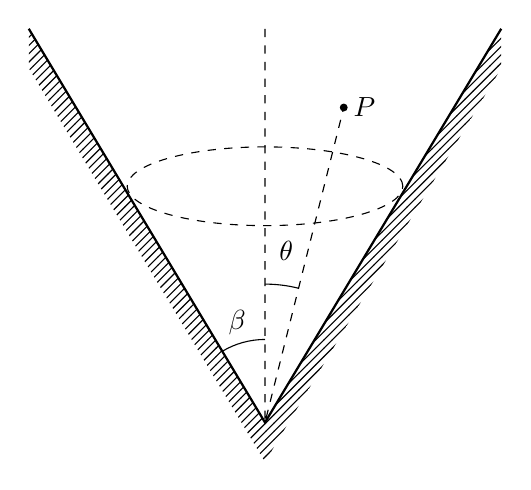
\begin{tikzpicture}
    \coordinate (o) at (0, 0);
    \coordinate (z) at (0, 5);
    \coordinate (a) at (3, 5);
    \coordinate (b) at (-3, 5);
    \coordinate (p) at (1, 4);
    \fill[pattern=north east lines](b)--(o)--(a)--(3, 4.5)--(0, -.5)--(-3, 4.5);
    \draw[thick](a)--(o)--(b);
    \draw[dashed](z)--(o)--(p);
    \draw[dashed](0, 3)ellipse(1.75 and .5);
    \fill(p)circle(.05)node[right]{$P$};
    \pic[draw, angle radius=30, angle eccentricity=1.25, "$\beta$"]{angle=z--o--b};
    \pic[draw, angle radius=50, angle eccentricity=1.25, "$\theta$"]{angle=p--o--z};
\end{tikzpicture}

\label{cylindrical boundary}
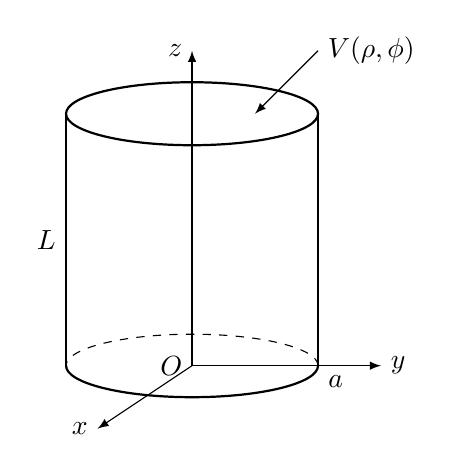
\begin{tikzpicture}[scale=.8]
    \draw[<->](0, 5)node[left]{$z$}--(0, 0)node[left]{$O$}--(3, 0)node[right]{$y$};
    \draw[->](0, 0)--(-1.5, -1)node[left]{$x$};
    \draw[dashed](2, 0)arc(0:180:2 and .5);
    \draw[thick](-2, 0)arc(-180:0:2 and .5);
    \draw[thick](0, 4)ellipse(2 and .5);
    \draw[thick](2, 0)node[below right]{$a$}--(2, 4);
    \draw[thick](-2, 0)--(-2, 4)node[midway, left]{$L$};
    \draw[<-](1, 4)--(2, 5)node[right]{$V(\rho,\phi)$};
\end{tikzpicture}

\label{concentric spheres boundary}
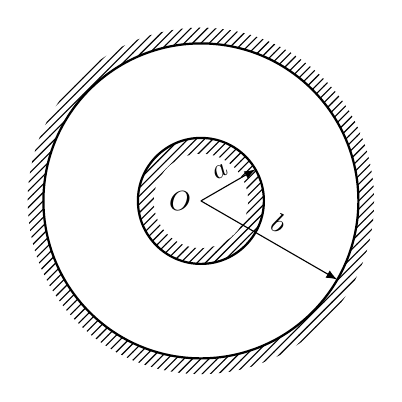
\begin{tikzpicture}[even odd rule]
    \coordinate[label=left:$O$](O)at(0, 0);
    \fill[pattern=north east lines](O)circle(2.2)(O)circle(2)(O)circle(.8)(O)circle(.6);
    \draw[thick](O)circle(.8)(O)circle(2);
    \draw[->](O)--(30:.8)node[midway, sloped, above]{$a$};
    \draw[->](O)--(-30:2)node[midway, sloped, above]{$b$};
\end{tikzpicture}

\label{method of images, dielectrics}
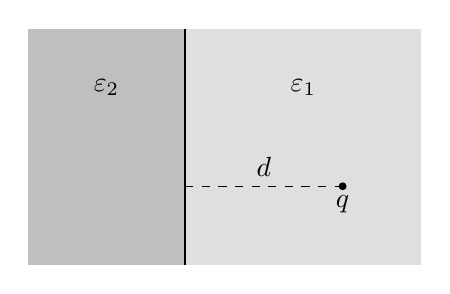
\begin{tikzpicture}
    \fill[gray!25](0, 0)rectangle(3, 3);
    \fill[gray!50](0, 0)rectangle(-2, 3);
    \node at(1.5, 2.25){$\varepsilon_1$};
    \node at(-1, 2.25){$\varepsilon_2$};
    \draw[thick](0, 0)--(0, 3);
    \draw[dashed](0, 1)--(2, 1)node[midway, above]{$d$};
    \fill[black](2, 1)circle(.05)node[below]{$q$};
\end{tikzpicture}

\label{H between magnetic surfaces}
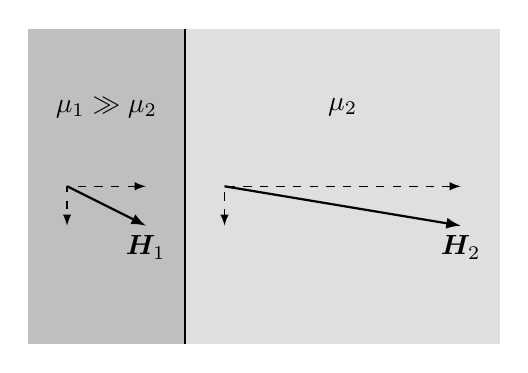
\begin{tikzpicture}
    \fill[gray!25](0, 0)rectangle(4, 4);
    \fill[gray!50](0, 0)rectangle(-2, 4);
    \node at(-1, 3){$\mu_1\gg\mu_2$};
    \node at(2, 3){$\mu_2$};
    \draw[thick](0, 0)--(0, 4);
    \draw[dashed, <->](-.5, 2)--(-1.5, 2)--(-1.5, 1.5);
    \draw[thick, ->](-1.5, 2)--(-.5, 1.5)node[below]{$\bm H_1$};
    \draw[dashed, <->](3.5, 2)--(.5, 2)--(.5, 1.5);
    \draw[thick, ->](.5, 2)--(3.5, 1.5)node[below]{$\bm H_2$};
\end{tikzpicture}

\label{linear polarization}
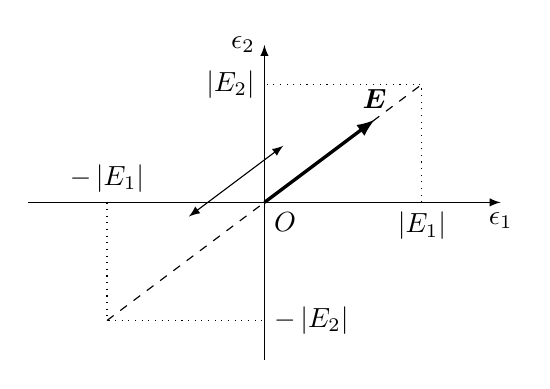
\begin{tikzpicture}
    \coordinate(O)at(0, 0);
    \coordinate(x)at(3, 0);
    \coordinate(y)at(0, 2); 
    \coordinate(E)at(2, 1.5); 
    \draw[->](-3, 0)--(x)node[below]{$\epsilon_1$};
    \draw[->](0, -2)--(y)node[left]{$\epsilon_2$};
    \node[below right]at(O){$O$};
    \draw[dashed](-2, -1.5)--(E);
    \draw[dotted](-2, 0)node[above]{$-\abs{E_1}$}--(-2, -1.5)--(0, -1.5)node[right]{$-\abs{E_2}$};
    \draw[dotted](2, 0)node[below]{$\abs{E_1}$}--(E)--(0, 1.5)node[left]{$\abs{E_2}$};
    \draw[very thick, ->, scale=0.7](O)--(2, 1.5)node[above]{$\bm E$};
    \draw[<->, scale=0.3, shift={(-1.2, 0.9)}](-2, -1.5)--(2, 1.5);
    % \pic[draw, angle radius=15, angle eccentricity=1.5, "$\delta$"]{angle=x--O--E};
\end{tikzpicture}

\label{circular polarization}
\begin{tikzpicture}[scale=.8]
    \draw[->](-3, 0)--(3, 0)node[below]{$\epsilon_1$};
    \draw[->](0, -3)--(0, 3)node[left]{$\epsilon_2$};
    \draw[dashed](0, 0)node[above left]{$O$}circle(2);
    \node[below]at(2, 0) {$\abs{E_1}$};
    \draw[very thick, ->](0, 0)--(45:2)node[above]{$\bm E$};
    \draw[->](30:2.6)arc(30:60:2.6);
\end{tikzpicture}

\label{elliptical polarization}
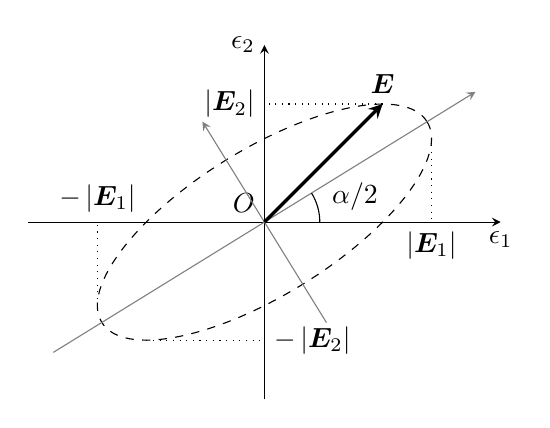
\begin{tikzpicture}[scale=1.5, >=stealth]
    \coordinate(O)at(0, 0);
    \coordinate(x)at(2, 0);
    \coordinate(a)at(31.68:2.5);
    \draw[->](-2, 0)--(x)node[below]{$\epsilon_1$};
    \draw[->](0, -1.5)--(0, 1.5)node[left]{$\epsilon_2$};
    \node[above left]at(O){$O$};
    \draw[dashed, rotate=31.68](O)ellipse[x radius=1.618, y radius=.618];
    \draw[->, gray, rotate=31.68](-2.1, 0)--(2.1, 0);
    \draw[->, gray, rotate=31.68](0, -1)--(0, 1);
    \draw[dotted](1.414, .707)--(1.414, 0)node[below]{$\abs{\bm E_1}$};
    \draw[dotted](-1.414, -.707)--(-1.414, 0)node[above]{$-\abs{\bm E_1}$};
    \draw[dotted](1, 1)--(0, 1)node[left]{$\abs{\bm E_2}$};
    \draw[dotted](-1, -1)--(0, -1)node[right]{$-\abs{\bm E_2}$};
    \draw[very thick, ->](0, 0)--(1, 1)node[above]{$\bm E$};
    \pic[draw, angle radius=20, angle eccentricity=1.7, "$\alpha/2$"]{angle=x--O--a};
\end{tikzpicture}

\label{reflection and transmission}
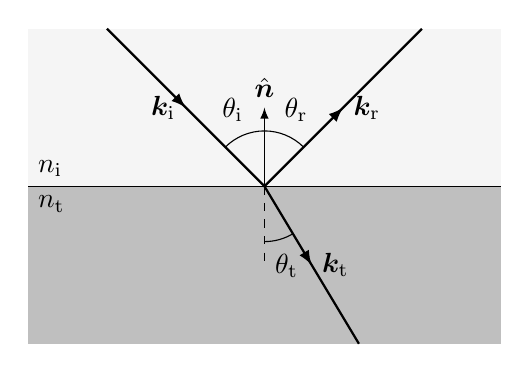
\begin{tikzpicture}
    \coordinate(O)at(0, 0);
    \coordinate(n)at(0, 1);
    \coordinate(u)at(0, -1);
    \coordinate(i)at(-2, 2);
    \coordinate(r)at(2, 2);
    \coordinate(t)at(1.2, -2);
    \fill[gray!8](-3, 0)rectangle(3, 2);
    \fill[gray!50](-3, 0)rectangle(3, -2);
    \draw(-3, 0)node[above right]{$n_\i$}node[below right]{$n_\t$}--(3, 0);
    \draw[dashed](O)--(u);
    \draw[->](O)--(n)node[above]{$\hat{\bm n}$};
    \draw[thick, ->-](O)--(r)node[midway, right]{$\bm k_\r$};
    \draw[thick, ->-](i)--(O)node[midway, left]{$\bm k_\i$};
    \draw[thick, ->-](O)--(t)node[midway, right]{$\bm k_\t$};
    \pic["$\theta_\i$", draw, angle radius=20, angle eccentricity=1.5]{angle=n--O--i};
    \pic["$\theta_\r$", draw, angle radius=20, angle eccentricity=1.5]{angle=r--O--n};
    \pic["$\theta_\t$", draw, angle radius=20, angle eccentricity=1.5]{angle=u--O--t};
\end{tikzpicture}

\label{Stokes relations}
\begin{tikzpicture}
    \fill[gray!8](-3, 0)rectangle(3, 2);
    \fill[gray!50](-3, 0)rectangle(3, -2);
    \draw(-3, 0)node[above right]{$n_1$}node[below right]{$n_2$}--(3, 0);
    \draw[dashed](n)--(u);
    \draw[thick, ->-](i)--(O)node[midway, below left]{$1$};
    \draw[thick, ->-](O)--(r)node[midway, below right]{$r_{12}$};
    \draw[thick, ->-](O)--(t)node[midway, above right]{$t_{12}$};
\end{tikzpicture}

\begin{tikzpicture}
    \coordinate(tr)at(-1.2, -2);
    \fill[gray!8](-3, 0)rectangle(3, 2);
    \fill[gray!50](-3, 0)rectangle(3, -2);
    \draw(-3, 0)node[above right]{$n_1$}node[below right]{$n_2$}--(3, 0);
    \draw[dashed](n)--(u);
    \draw[thick, ->-, red](r)--(O)node[midway, below right]{$r_{12}$};
    \draw[thick, ->-, red]([shift={(-.1, 0)}]O)--([shift={(-.1, 0)}]i)node[midway, below left]{$r_{12}^2$};
    \draw[dashed, ->-, red]([shift={(-.1, 0)}]O)--([shift={(-.1, 0)}]tr)node[midway, above left]{$r_{12}t_{12}$};
    \draw[thick, ->-, blue](t)--(O)node[midway, above right]{$t_{12}$};
    \draw[thick, ->-, blue](O)--(i)node[midway, above right]{$t_{12}t_{21}$};
    \draw[dashed, ->-, blue](O)--(tr)node[midway, below right]{$t_{12}r_{21}$};
\end{tikzpicture}

\label{perpendicular polarization}
\begin{tikzpicture}
    \coordinate(t)at(1.5, -2.5);
    \coordinate(Ei)at(-1.2, 1.2);
    \coordinate(Er)at(1, 1);
    \coordinate(Et)at(.6, -1);
    \fill[gray!8](-3, 0)rectangle(3, 2);
    \fill[gray!50](-3, 0)rectangle(3, -2.5);
    \draw(-3, 0)node[above right]{$n_\i$}node[below right]{$n_\t$}--(3, 0);
    \draw[dashed](n)--(u);
    \draw(O)--(r);
    \draw(i)--(O);
    \draw(O)--(t);
    % incident
    \draw[thick, ->](Ei)--(-.7, .7)node[shift={(30:.3)}]{$\bm k_\i$};
    \draw[thick, ->](Ei)--(-1.7, .7)node[left]{$\bm H_\i$};
    \draw[thick, fill=white](Ei)circle(.12)node[shift={(30:.4)}]{$\bm E_\i$};
    \fill[black](Ei)circle(.06);
    % reflect
    \draw[thick, ->](Er)--(1.5, 1.5)node[shift={(150:.3)}]{$\bm k_\r$};
    \draw[thick, ->](Er)--(1.5, .5)node[right]{$\bm H_\r$};
    \draw[thick, fill=white](Er)circle(.12)node[shift={(150:.4)}]{$\bm E_\r$};
    \fill[black](Er)circle(.06);
    % transmit
    \draw[thick, ->](Et)--(1.2, -2)node[right]{$\bm k_\t$};
    \draw[thick, ->](Et)--(.1, -1.3)node[left]{$\bm H_\t\!$};
    \draw[thick, fill=white](Et)circle(.12)node[right]{$\bm E_\t$};
    \fill[black](Et)circle(.06);
\end{tikzpicture}

\label{parallel polarization}
\begin{tikzpicture}
    \fill[gray!8](-3, 0)rectangle(3, 2);
    \fill[gray!50](-3, 0)rectangle(3, -2.5);
    \draw(-3, 0)node[above right]{$n_\i$}node[below right]{$n_\t$}--(3, 0);
    \draw[dashed](n)--(u);
    \draw(O)--(r);
    \draw(i)--(O);
    \draw(O)--(t);
    % incident
    \draw[thick, ->](Ei)--(-.7, .7)node[shift={(30:.3)}]{$\bm k_\i$};
    \draw[thick, ->](Ei)--(-.7, 1.7)node[right]{$\bm E_\i$};
    \draw[thick, fill=white](Ei)circle(.12)node[shift={(210:.4)}]{$\bm H_\i$};
    \fill[black](Ei)circle(.06);
    % reflect
    \draw[thick, ->](Er)--(1.5, 1.5)node[shift={(-30:.3)}]{$\bm k_\r$};
    \draw[thick, ->](Er)--(.5, 1.5)node[shift={(150:.3)}]{$\bm E_\r$};
    \draw[thick, fill=white](Er)circle(.12)node[shift={(-30:.4)}]{$\bm H_\r$};
    \fill[black](Er)circle(.06);
    % transmit
    \draw[thick, ->](Et)--(1.2, -2)node[right]{$\bm k_\t$};
    \draw[thick, ->](Et)--(1.1, -.7)node[right]{$\bm E_\t$};
    \draw[thick, fill=white](Et)circle(.12)node[shift={(210:.4)}]{$\bm H_\t$};
    \fill[black](Et)circle(.06);
\end{tikzpicture}

\label{rectangular waveguide}
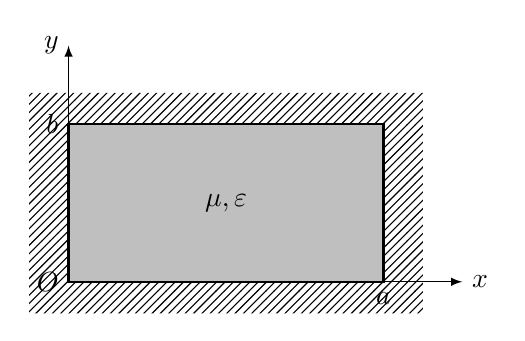
\begin{tikzpicture}[even odd rule]
    \fill[pattern=north east lines](-.5, -.4)rectangle(4.5, 2.4)(0, 0)rectangle(4, 2);
    \draw[thick, fill=gray!50](4, 0)node[below]{$a$}rectangle(0, 2)node[left]{$b$};
    \node at (2, 1) {$\mu,\varepsilon$};
    \draw[<->](0, 3)node[left]{$y$}--(0, 0)node[left]{$O$}--(5, 0)node[right]{$x$};
\end{tikzpicture}

\label{circle waveguide}
\begin{tikzpicture}[even odd rule]
    \coordinate(x)at(2, 0);
    \coordinate(P)at(60:1.5);
    \fill[pattern=north east lines](O)circle(2)(O)circle(2.2);
    \draw[thick, fill=gray!50](O)circle(2);
    \node at (0, -1) {$\mu,\varepsilon$};
    \draw[dashed](O)--(x)node[midway, below]{$a$};
    % \draw(O)--(P)node[midway, left]{$\rho$};
    % \pic["$\phi$", draw, angle radius=20, angle eccentricity=1.5]{angle=x--O--P};
\end{tikzpicture}

\label{dielectric waveguide}
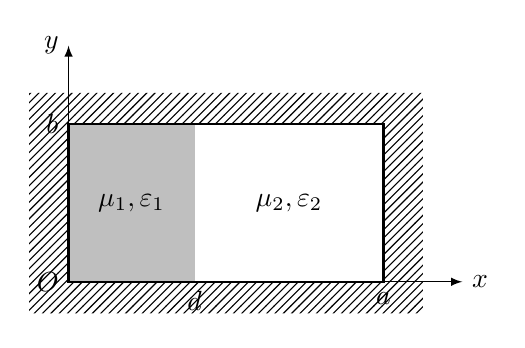
\begin{tikzpicture}[even odd rule]
    \fill[pattern=north east lines](-.5, -.4)rectangle(4.5, 2.4)(0, 0)rectangle(4, 2);
    \fill[gray!50](0, 0)rectangle(1.6, 2);
    \node at (1.6, 0) [below] {$d$};
    \draw[thick](4, 0)node[below]{$a$}rectangle(0, 2)node[left]{$b$};
    \node at (0.8, 1) {$\mu_1,\varepsilon_1$};
    \node at (2.8, 1) {$\mu_2,\varepsilon_2$};
    \draw[<->](0, 3)node[left]{$y$}--(0, 0)node[left]{$O$}--(5, 0)node[right]{$x$};
\end{tikzpicture}

\label{Michelson-Morley experiment}
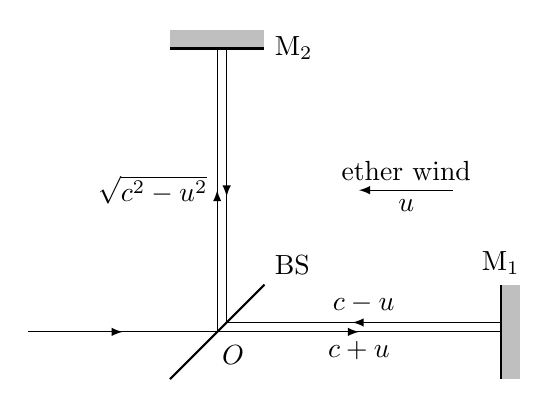
\begin{tikzpicture}[scale=1.2]
    \draw[->-](0, 0)--(2, 0)node[shift={(.2, -.3)}]{$O$};
    \draw[thick](2-.5, -.5)--(2.5, .5)node[above right]{BS};
    \draw[->-](2, 0)--(5, 0)node[midway, below]{$c+u$};
    \draw[-<-](2.1, .1)--(5, .1)node[midway, above]{$c-u$};
    \fill[gray!50](5, .5)rectangle(5.2, -.5);
    \draw[thick](5, -.5)--(5, .5)node[above]{M$_1$};
    \draw[->-](2, 0)--(2, 3)node[midway, left]{$\sqrt{c^2-u^2}$};
    \draw[-<-](2.1, .1)--(2.1, 3);
    \fill[gray!50](1.5, 3)rectangle(2.5, 3.2);
    \draw[thick](1.5, 3)--(2.5, 3)node[right]{M$_2$};
    \draw[<-](3.5, 1.5)--(4.5, 1.5)node[midway, below]{$u$}node[midway, above]{ether wind};
\end{tikzpicture}

\label{Compton scattering}
\begin{tikzpicture}
    \coordinate (O) at (0, 0);
    \coordinate (x) at (3, 0);
    \coordinate (v) at (3, 2);
    \coordinate (e) at (2, -2);
    \draw[->, thick, gray, decorate, decoration={
        snake, amplitude=.4mm, segment length=2mm, post length=1mm}]
        (-3, 0)node[above]{$h\nu$}--(O);
    \draw[->, thick, decorate, decoration={
        snake, amplitude=.4mm, segment length=4mm, post length=1mm}]
        (O)--(v)node[right]{$h\nu'$};
    \draw[->, thick](O)--(e)node[right]{e$^-$};
    \draw[dashed](O)--(x);
    \pic[draw, "$\theta$", angle radius=8mm, angle eccentricity=1.2]{angle=x--O--v};
    \pic[draw, "$\phi$", angle radius=10mm, angle eccentricity=1.2]{angle=e--O--x};
\end{tikzpicture}

\label{q in lab frame}
\begin{tikzpicture}[xscale=.8]
    \draw[->, thick](-3, 2.3)node[left]{$\lambda_+$}--(-2, 2.3)node[right]{$\bm v_+$};
    \draw[->, thick](3, 1.7)node[right]{$\lambda_-$}--(2, 1.7)node[left]{$\bm v_-$};
    \draw[thick](-3, 2)--(3, 2);
    \draw[dashed](0, 0)--(0, 2)node[midway, right]{$r$};
    \draw[->, thick](0, 0)--(.5, 0)node[above]{$\bm u$};
    \fill[black](0, 0)circle(0.1)node[left]{$q$};
\end{tikzpicture}

\label{q in q frame}
\begin{tikzpicture}[xscale=.8]
    \draw[->, thick](-3, 2.3)node[left]{$\lambda_+'$}--(-2.2, 2.3)node[right]{$\bm v_+'$};
    \draw[->, thick](3, 1.7)node[right]{$\lambda_-'$}--(1.8, 1.7)node[left]{$\bm v_-'$};
    \draw[thick](-3, 2)--(3, 2);
    \draw[dashed](0, 0)--(0, 2)node[midway, right]{$r$};
    \fill[black](0, 0)circle(0.1)node[left]{$q$};
\end{tikzpicture}

\end{document}